\documentclass[11pt,a4paper]{article}
\usepackage[margin=20mm]{geometry}
\usepackage{graphicx,hyperref}
\renewcommand{\thefigure}{S\arabic{figure}}
\begin{document}
\section*{Supplement: Reinforcement patterns in the 16-rib reference}
Figure~S11 compares the saved core thickness after FSD with its final value and cumulative multiplication factor. The crop covers $y<8$~m and local chord fractions 0.70--0.95. Vertical lines mark rib planes. The periodic thickness features are inherited from stress sizing and amplified by multiplicative core growth. This is a saved-field diagnostic; it does not establish mesh independence or manufacturing feasibility.
\setcounter{figure}{10}
\begin{figure}[h]\centering
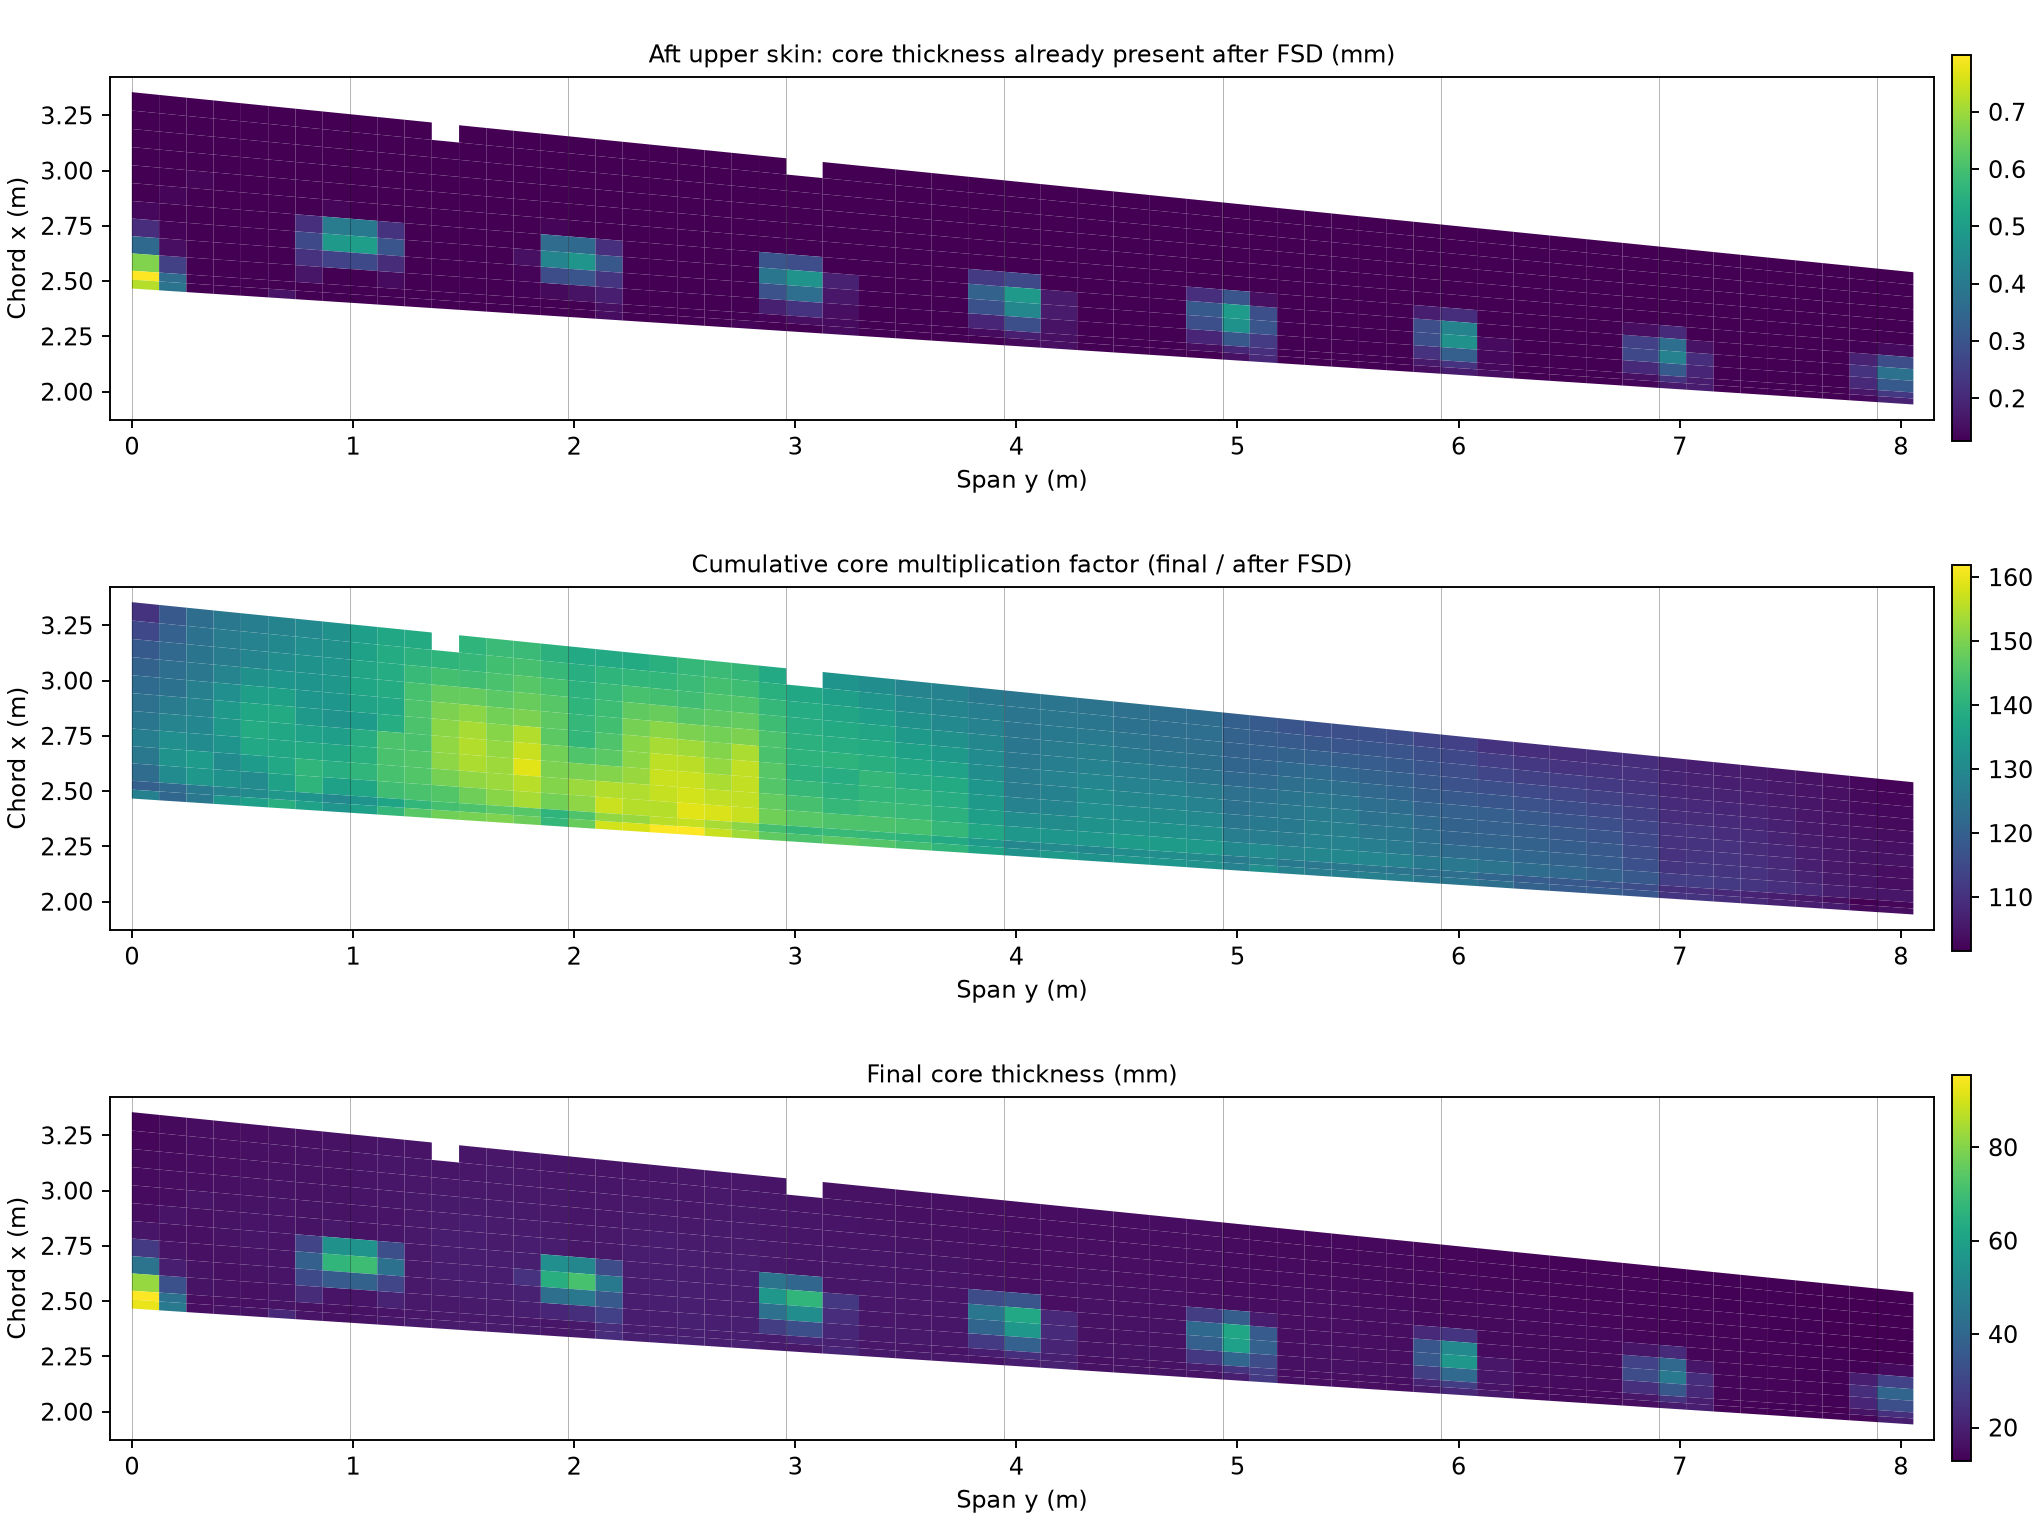
\includegraphics[width=\textwidth,height=.70\textheight,keepaspectratio]{aft_pattern_origin.png}
\caption{Aft upper-skin core field after FSD, accumulated core multiplication factor, and final core thickness. Each row uses its own units and scale. Polygons represent saved elements.}
\end{figure}
\clearpage
Figure~S12 shows the evolution of selected saved first-mode fields. Each displacement field is normalized by its upper-skin maximum absolute element-averaged normal displacement. Mode sign is arbitrary. Energy is normalized by its upper-skin maximum; the plotted logarithm is floored at $-12$. These visualizations use independent per-state normalization and do not compare absolute modal amplitudes between states.
\begin{figure}[h]\centering
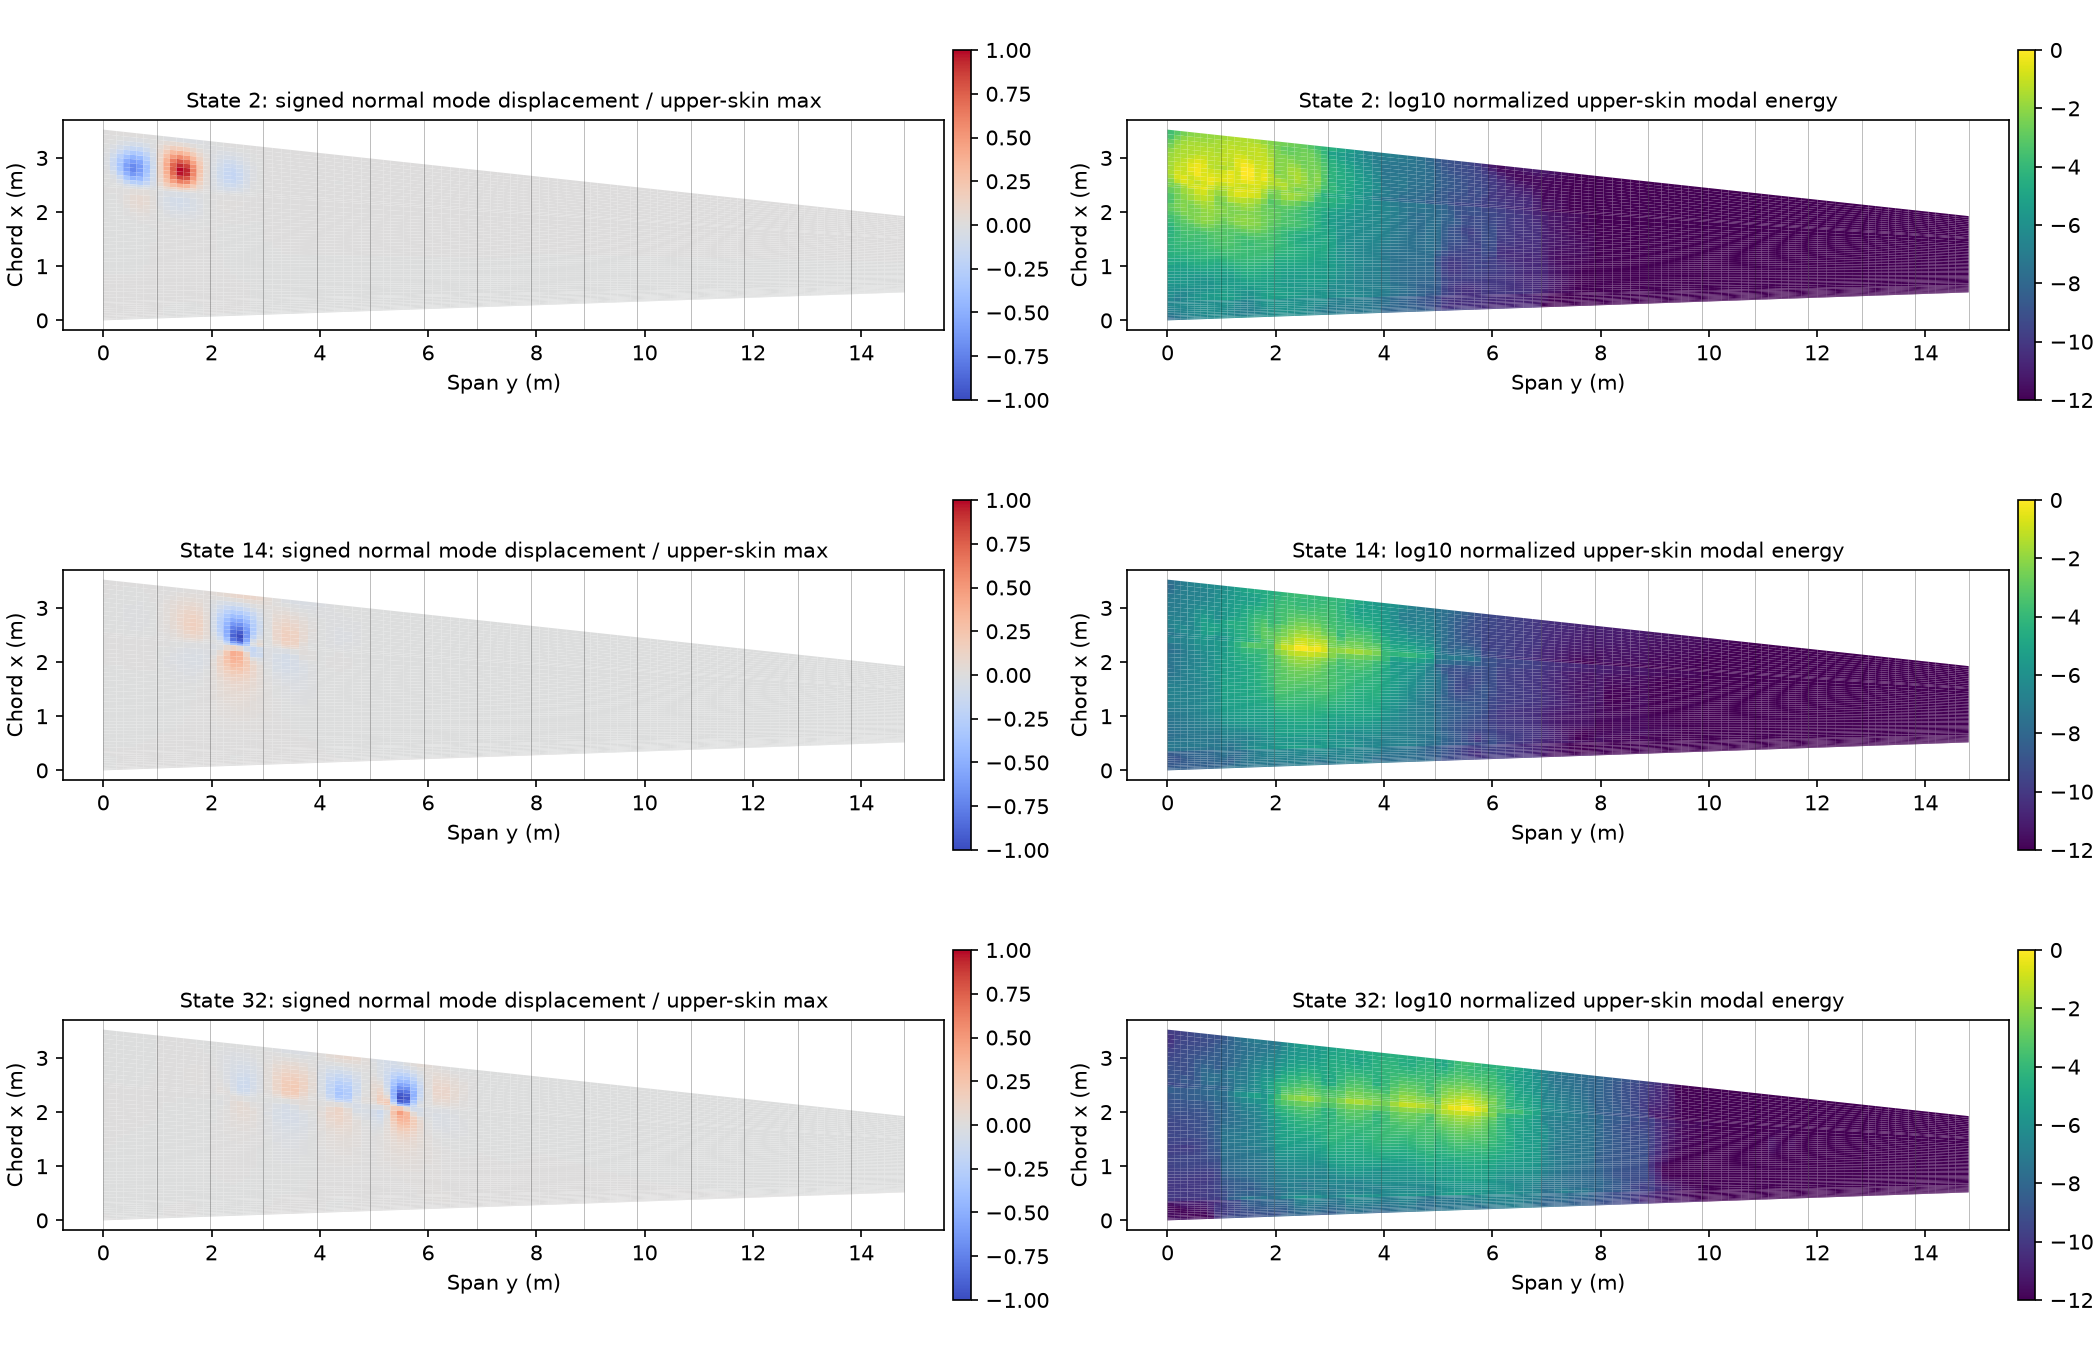
\includegraphics[width=\textwidth,height=.70\textheight,keepaspectratio]{saved_modes.png}
\caption{Upper-skin first-mode normal displacement and modal strain energy at states 2, 14 and 32. Vertical lines indicate rib stations. The accumulated thickness field reflects the full update history, not only the final mode.}
\end{figure}
\end{document}
